\chapter{Dokumentacja techniczna aplikacji ExpensePredictor}
\section{Opis wymagań funkcjonalnych aplikacji}
Wymagania funkcjonalne, które stworzony system ma spełniać uwzględniają czynności z zakresu zarządzania własnymi danymi, rejestracji przychodów i wydatków oraz predykcji wydatków, są przedstawione na diagramie przypadków użycia (Rys. \ref{usecases}) oraz opisane poniżej:
\begin{itemize}
	\item\textbf{rejestracja} - utworzenie nowego konta przez niezalogowanego użytkownika, 
	\item\textbf{logowanie} - proces generowania tokenu pozwalającego na dostęp do aplikacji ,
	\item\textbf{wyświetlanie danych użytkownika} - dostęp do podstawowych danych użytkownika, takich jak imię, nazwisko lub numer telefonu,
	\item\textbf{edycja danych użytkownika} - edycja podstawowych danych użytkownika,
	\item\textbf{zmiana hasła użytkownika} - zmiana hasła aktualnie zalogowanego użytkownika,
	\item\textbf{wyświetlenie listy wydatków} - dostęp do listy wszystkich wydatków aktualnie zalogowanego użytkownika z określonego okresu,
	\item\textbf{wyświetlenie danych wydatku} - dostęp do szczegółów wybranego wydatku,
	\item\textbf{dodanie wydatku} - dodanie nowego wydatku dla aktualnie zalogowanego użytkownika,
	\item\textbf{edycja wydatku} - zmiana kwoty, daty, kategorii i opisu istniejącego wydatku,
	\item\textbf{usunięcie wydatku} - usunięcie wybranego wydatku z listy wydatków aktualnie zalogowanego użytkownika,
	\item\textbf{wyświetlenie listy przychodów} - dostęp do listy wszystkich przychodów aktualnie zalogowanego użytkownika z określonego okresu,
	\item\textbf{wyświetlenie danych przychodu} - dostęp do szczegółów wybranego przychodu,
	\item\textbf{dodanie przychodu} - dodanie nowego przychodu dla aktualnie zalogowanego użytkownika,
	\item\textbf{edycja przychodu} - zmiana kwoty, daty, kategorii i opisu istniejącego przychodu,
	\item\textbf{usunięcie przychodu} - usunięcie wybranego przychodu z listy przychodów aktualnie zalogowanego użytkownika,
	\item\textbf{predykcja wydatków} - wykonanie prognozy wielkości wydatków powiązanych z wydatkiem głównym na nadchodzące miesiące,
	\item\textbf{dodanie kategorii wydatków lub przychodów} - dodanie przez administratora kategorii, do której użytkownicy mogą przypisywać swoje wydatki lub przychody,
	\item\textbf{edycja kategorii wydatków lub przychodów} - zmiana przez administratora opisu istniejącej kategorii wydatków lub przychodów.
\end{itemize}
\begin{figure}[!ht]
	\begin{center}
		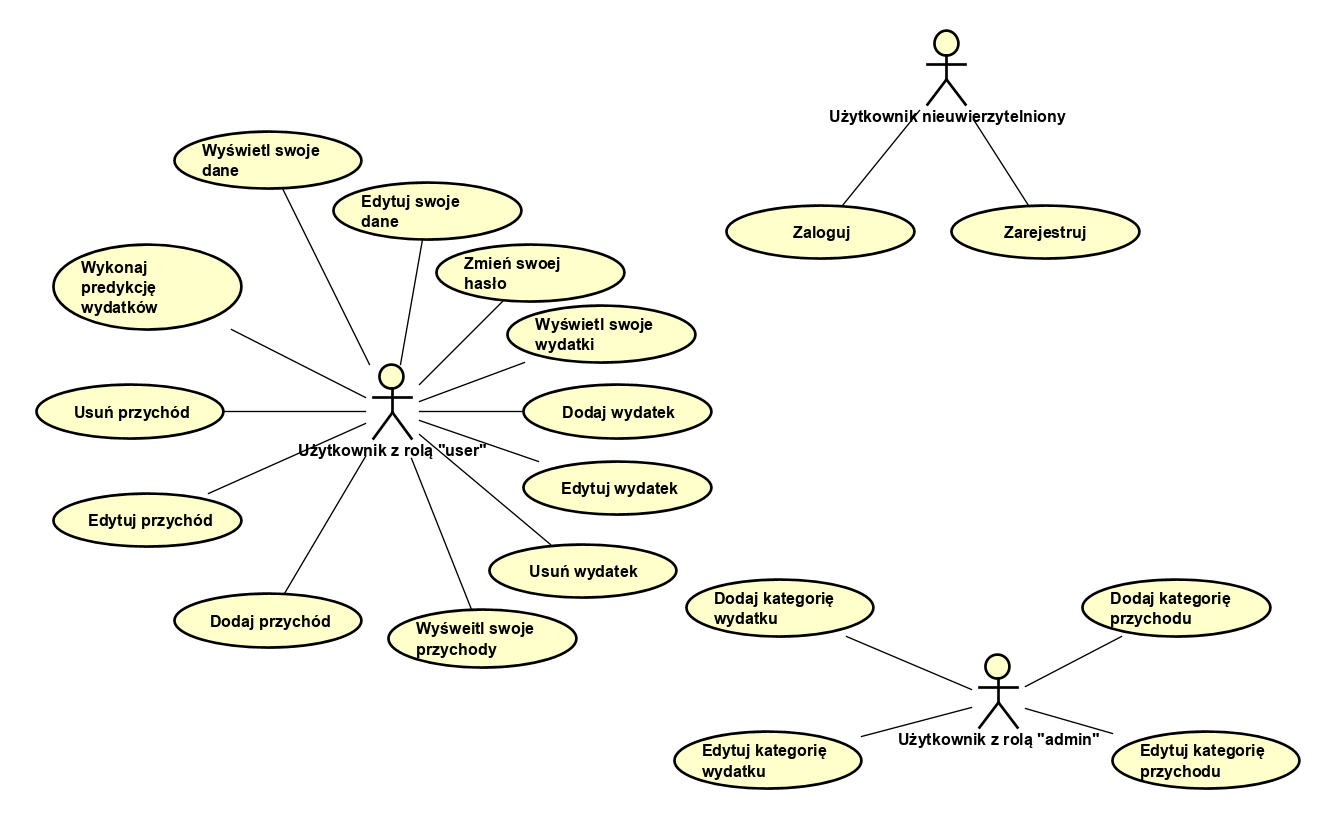
\includegraphics[width=6in]{img/diagram/use_cases.png}
		\caption{Diagram przypadków użycia}
		\label{usecases}
	\end{center}
\end{figure}
\section{Opis wymagań niefunkcjonalnych aplikacji}
Wymagania niefunkcjonalne uwzględniają ograniczenia systemu z zakresu bezpieczeństwa lub optymalizacji:
\begin{itemize}
	\item\textbf{bezpieczne hasło} - nałożenie ograniczeń, które ciąg znaków musi spełniać, aby mógł być użyty jako hasło: minimalna długość to osiem znaków, ciąg musi zawierać co najmniej jedną małą i dużą literę, liczbę oraz znak specjalny,
	\item\textbf{dostęp do systemu dla uwierzytelnionych użytkowników} - możliwość skorzystania z funkcjonalności systemu (z kilkoma wyjątkami) jest dostępna jedynie dla uwierzytelnionych użytkowników,
	\item\textbf{dostęp do funkcjonalności ograniczony rolami} - dostęp do funkcjonalności jest ograniczony poprzez role przypisane do konta użytkownika, na przykład edycję kategorii wykonać może jedynie użytkownik, który posiada rolę "admin",
	\item\textbf{użycie tokenu} - wykorzystanie do uwierzytelniania i autoryzacji tokenu, który przechowuje informacje na temat tożsamości użytkownika oraz jego ról po stronie aplikacji klienckiej,
	\item\textbf{przechowywanie hasła w postaci jego skrótu} - wykorzystanie funkcji skrótu (ang. \textit{hash function}), aby nie przechowywać hasła w bazie danych w postaci jawnej,
	\item\textbf{tworzenie modelu regresji przy starcie aplikacji} - wyznaczenie współczynników regresji przed skorzystaniem z funkcjonalności predykcji przez użytkownika, gdyż operacja ta jest czasochłonna przy dużej ilości danych,
	\item\textbf{obsługa błędów} - wyświetlenie użytkownikowi komunikatu z opisem błędu w razie jego wystąpienia.
\end{itemize}
\section{Warstwa modelu danych}
Warstwa modelu danych składa się z bazy danych, klas encyjnych oraz klas zapewniających podstawowe operacje na danych.

Dane w bazie danych (Rys. \ref{db_diagram}) podzielone są na siedem tabel:
\begin{itemize}
	\item\textbf{AspNetUsers} - zawiera dane o użytkownikach. Struktura tabeli wynika z mapowania wbudowanych w ASP.NET Core struktur służących do zarządzania użytkownikami.
	\item\textbf{AspNetRoles} - tabela zawierająca zdefiniowane w systemie role użytkowników.
	\item\textbf{AspNetUserRoles} - tabela definiująca powiązania między użytkownikami a ich rolami.
	\item\textbf{Incomes} - tabela zawierająca przychody wszystkich użytkowników. Jeden rekord zawiera takie dane jak użytkownik, do którego dany przychód należy, kwota przychodu, jego kategoria, data i opis.
	\item\textbf{IncomeCategories} - tabela z definicjami kategorii przychodów.
	\item\textbf{Expenses} - tabela zawierająca wydatki użytkowników. Zawiera ona koszt, kategorię, datę oraz opis wydatku, użytkownika, do którego należy oraz flagę określającą czy jest to główny wydatek.
	\item\textbf{ExpenseCategories} - tabela definiująca kategorie wydatków.
\end{itemize}
\begin{figure}[!ht]
	\begin{center}
		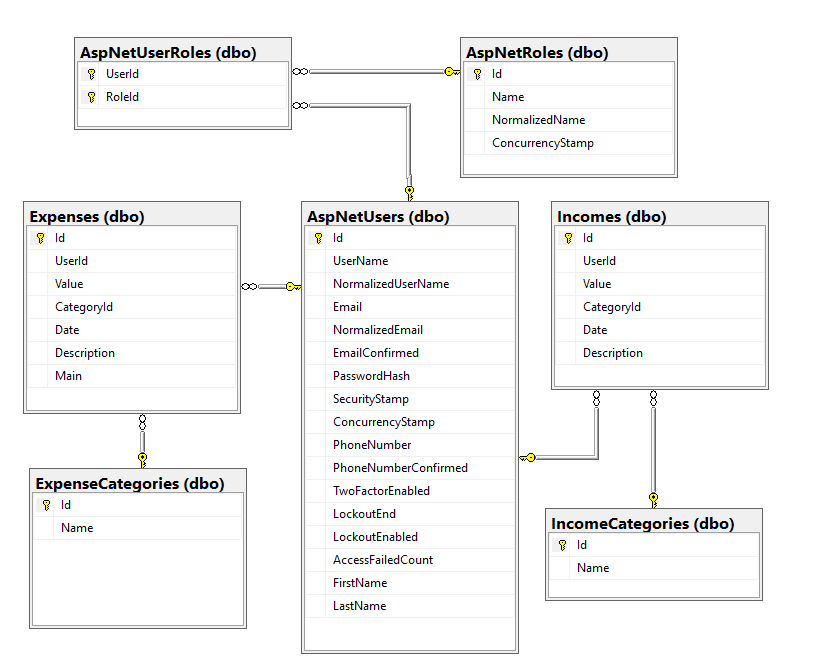
\includegraphics[width=6in]{img/diagram/db_diagram.png}
		\caption{Diagram bazy danych}
		\label{db_diagram}
	\end{center}
\end{figure}

Dostęp do danych w bazie danych z poziomu części serwerowej odbywa się przy pomocy klas encyjnych i mapowania relacyjno-obiektowego oraz klas zapewniających podstawowe operacje na danych. Diagram typów tej warstwy znajduje się na Rys. \ref{dal_dependecies}. Wszystkie klasy encyjne implementują interfejs \lstinline|IEntity| oraz odwzorowują strukturę bazy danych, a metody dostępu do danych dla pozostałych warstw aplikacji zapewnione są przez generyczny interfejs \lstinline|IApplicationRepository<TEntity>|, gdzie typ \lstinline|TEntity| obrazuje klasę encyjną (Rys. \ref{iapprepository}).\\
Dodatkowo w warstwie modelu danych znajduje się klasa \lstinline|DataInitializer|, która zawiera początkowe dane, jakie baza danych musi zawierać przy uruchomieniu aplikacji. Dane te są umieszczane w bazie podczas migracji, czyli procesu tworzącego strukturę bazy danych na podstawie istniejących klas encyjnych.
\begin{figure}[!ht]
\begin{center}
	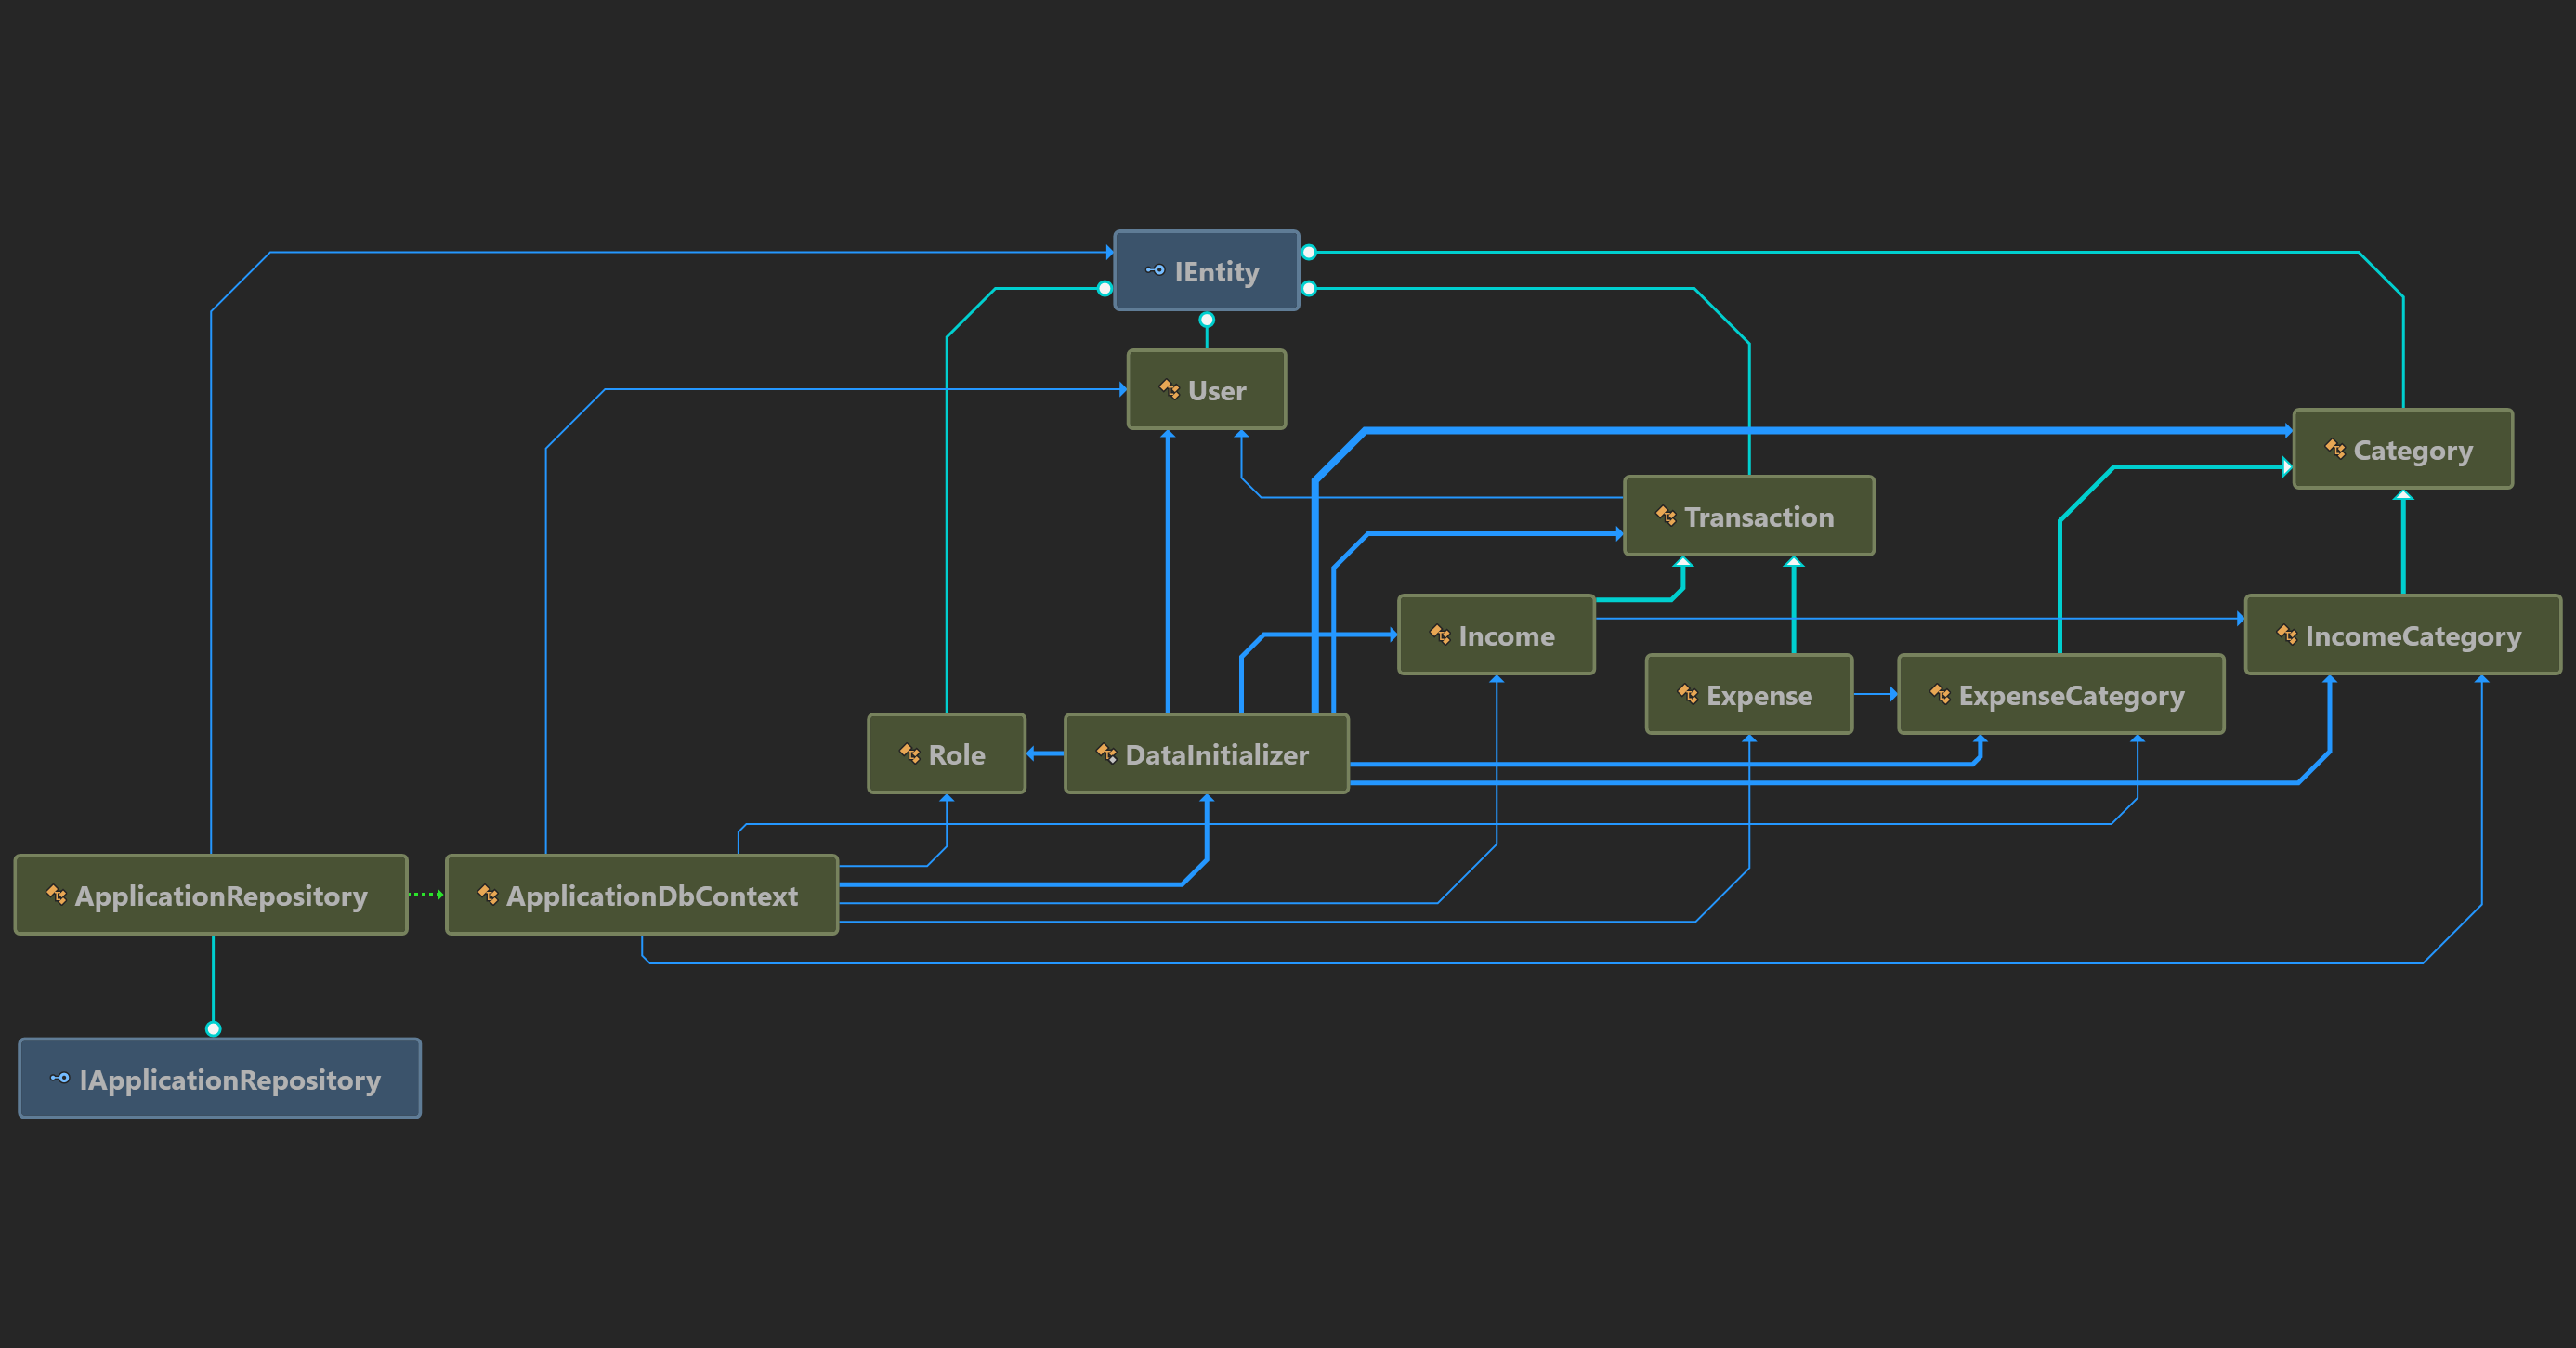
\includegraphics[width=6in]{img/diagram/dal_dependencies.png}
	\caption{Diagram zależności typów warstwy modelu danych}
	\label{dal_dependecies}
\end{center}
\end{figure}
\begin{figure}[!ht]
\begin{center}
	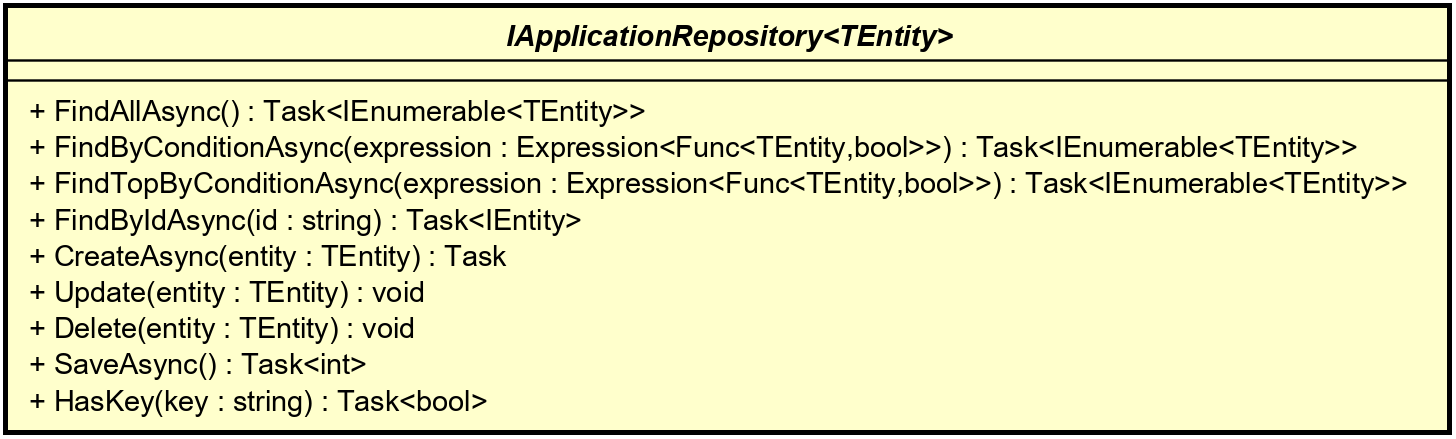
\includegraphics[width=6in]{img/diagram/iapprepository.png}
	\caption{Diagram interfejsu \lstinline|IApplicationRepository|}
	\label{iapprepository}
\end{center}
\end{figure}
\section{Warstwa logiki biznesowej}
Na warstwę logiki biznesowej składają się klasy realizujące logikę przypadków użycia, typy definiujące DTO i wyjątki aplikacyjne oraz klasy kontrolerów, pozwalających na dostęp do części serwerowej z poziomu aplikacji klienckiej.\\
W warstwie tej można wydzielić cztery moduły: moduł danych użytkownika, moduł wydatków, moduł przychodów oraz moduł predykcji. Na Rys. \ref{expensediagram} przedstawiony jest diagram klas modułu wydatków, pozostałe moduły posiadają analogiczną strukturę.
\begin{figure}[!ht]
	\begin{center}
		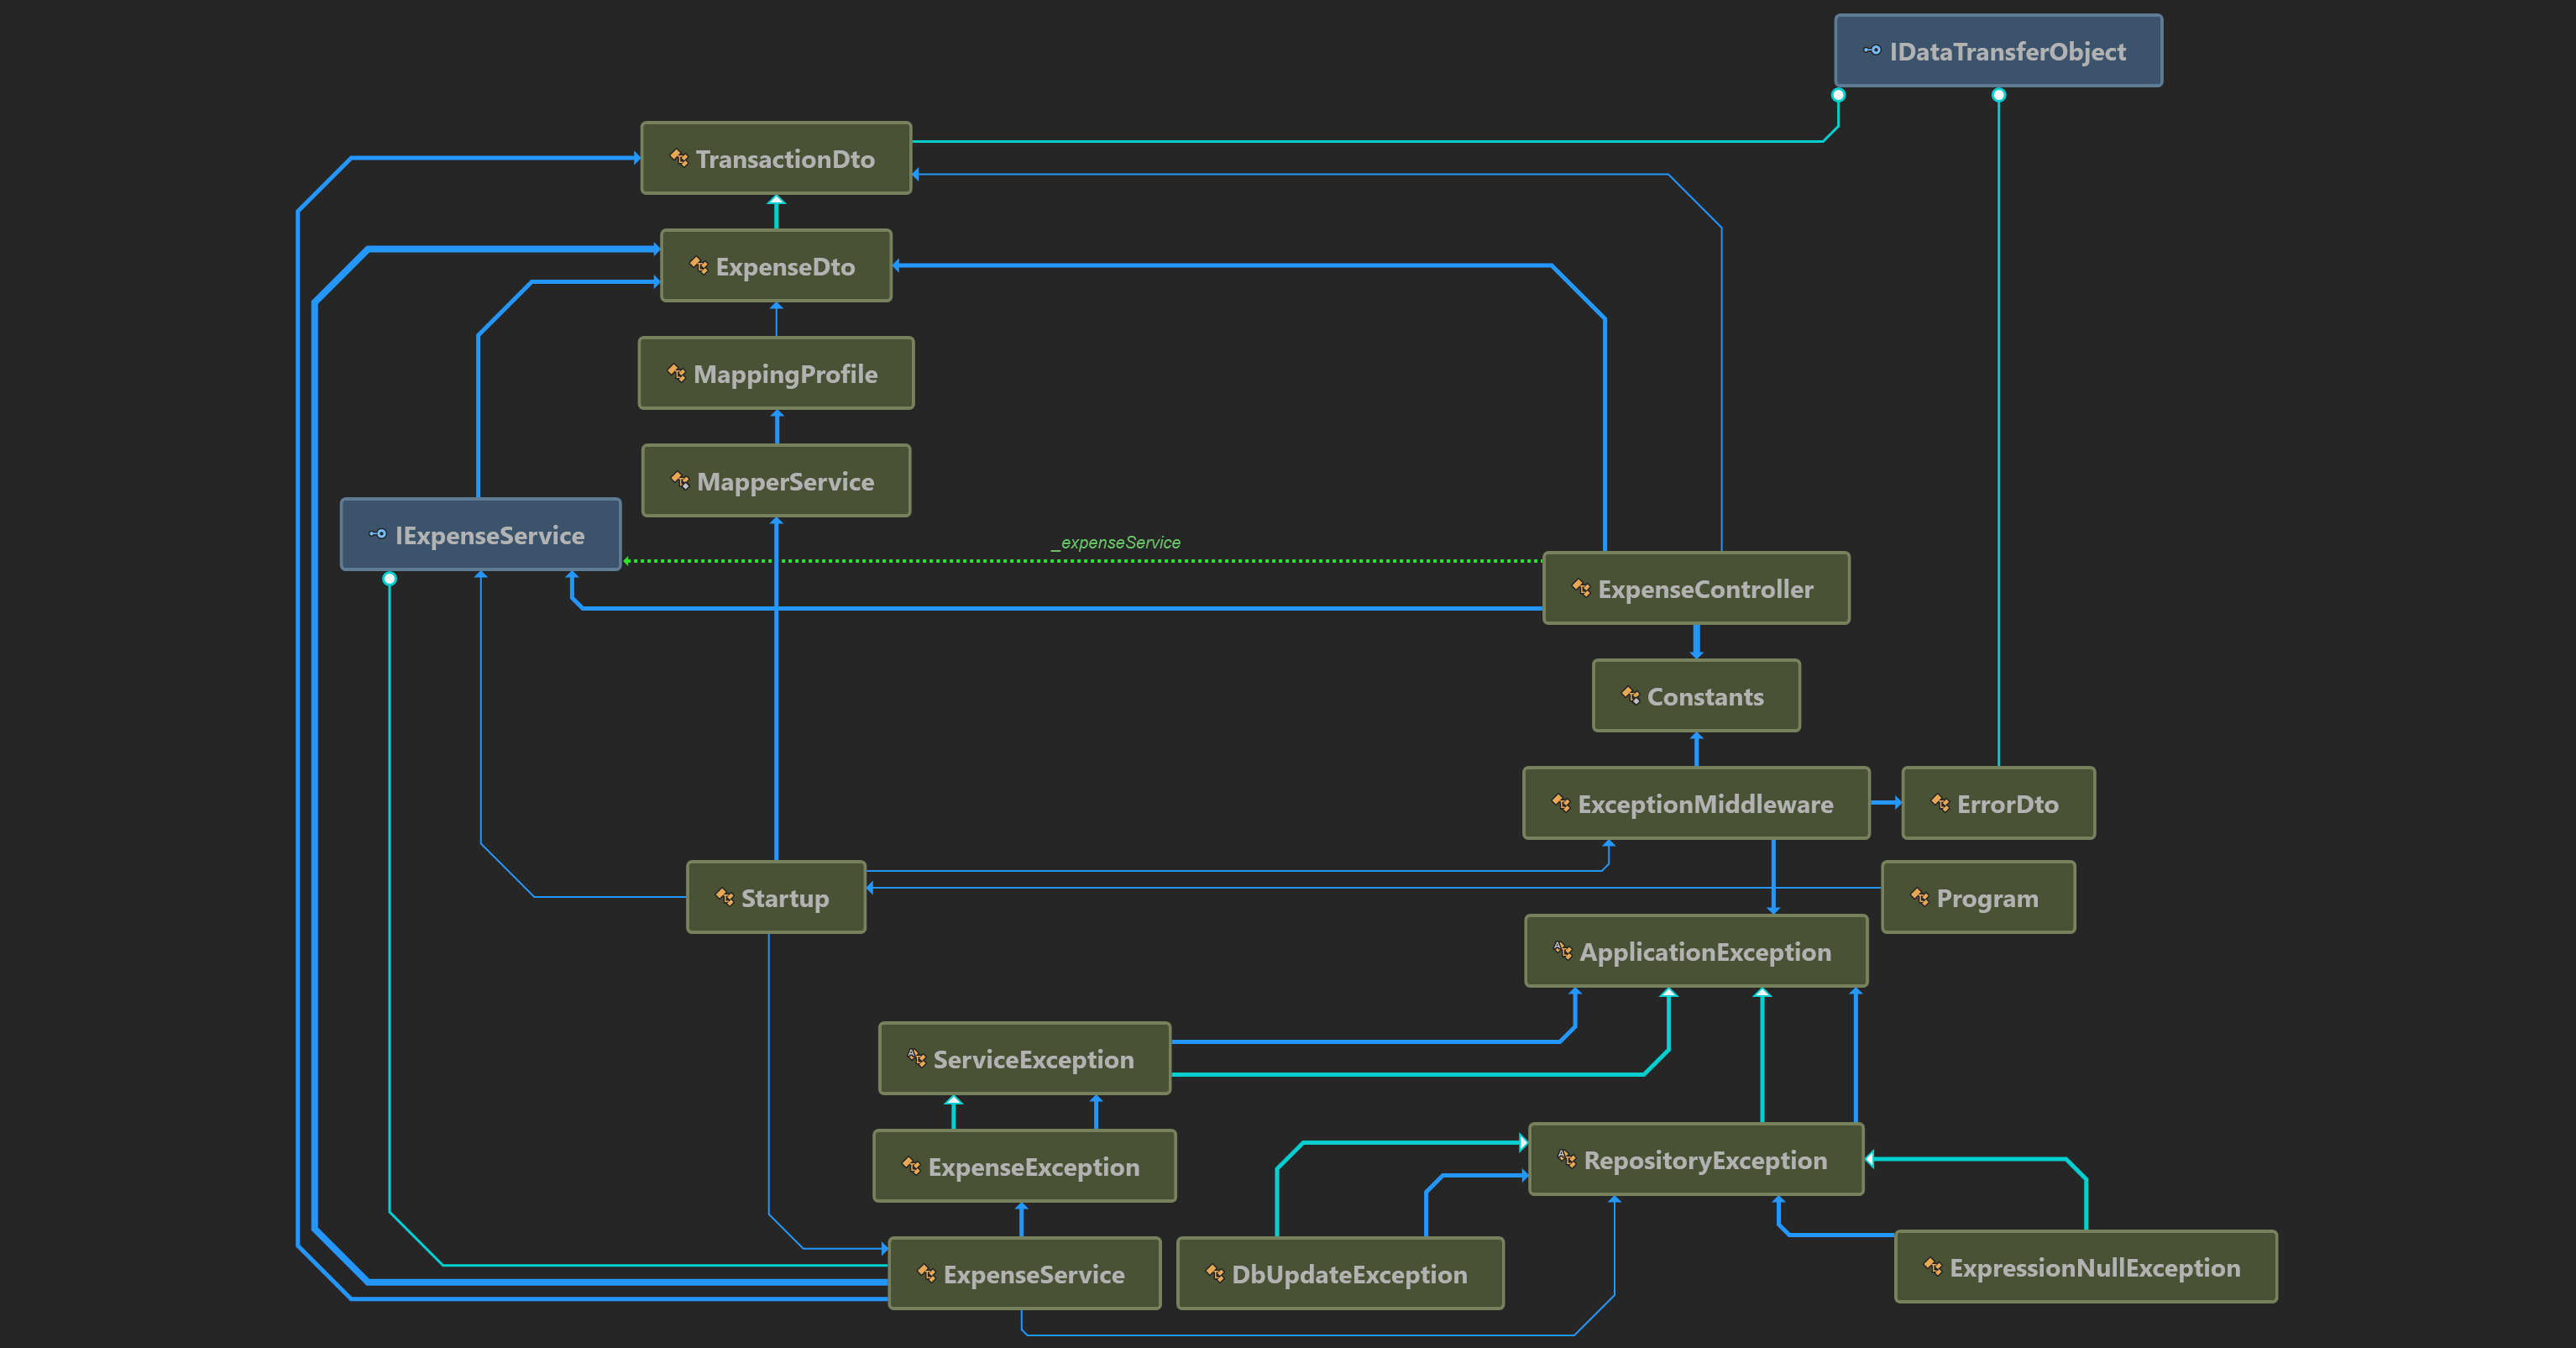
\includegraphics[width=6in]{img/diagram/expense_diagram.png}
		\caption{Diagram zależności typów warstwy logiki biznesowej dla modułu wydatków.}
		\label{expensediagram}
	\end{center}
\end{figure}

Wszystkie operacje poza logowaniem oraz rejestracją wymagają od użytkownika podania tokenu uwierzytelniającego. Następnie przebiega weryfikacja tokenu, czyli sprawdzenie podpisu cyfrowego w celu stwierdzenia, czy nie został on zmieniony bądź wygenerowany w inny sposób niż przy procesie logowania lub rejestracji oraz zweryfikowanie, czy użytkownik posiada role wymagane do wykonania danej operacji.

W celu rejestracji, po otrzymaniu danych o nowym koncie od użytkownika, przy pomocy zapewnionej przez ASP .NET Core klasy \lstinline|UserManager| tworzony jest nowe konto. Po utworzeniu użytkownika przypisywane są do niego role początkowe. Jeżeli proces rejestracji przebiegł pomyślnie, generowany jest token oraz zwracany użytkownikowi, przez co po rejestracji logowanie przebiega automatycznie.

Logowanie istniejącego użytkownika polega na wygenerowaniu dla niego tokenu uwierzytelniającego go w systemie. Po otrzymaniu danych w postaci loginu oraz hasła, są one weryfikowane. Przy pomyślnej weryfikacji odczytywane są z bazy danych wszystkie role przypisane do użytkownika i wraz z innymi danymi o użytkowniku zapisywane tokenie. Wygenerowany token jest podpisywany cyfrowo, co pozwala na jego weryfikację przy próbie uwierzytelnienia i odrzucenie w razie wykrycia jakiejkolwiek ingerencji w jego zawartość.

Zmiana hasła użytkownika wymaga podania starego oraz nowego hasła. Po weryfikacji poprawności dotychczasowego hasła generowany jest skrót nowego hasła, który zastępuje istniejący skrót. Oprócz zmiany hasła użytkownik może także zmienić swoje dane osobowe.

Dodawanie i edycja kategorii są dostępne jedynie dla użytkownika posiadającego rolę "admin". Operacje te sprowadzają się do zmodyfikowania bądź stworzenia rekordu w bazie danych zawierającego opis danej kategorii. Raz stworzonej kategorii nie można usunąć z powodu powiązanych z nią wydatków bądź dochodów użytkowników.

Dodawanie wydatku lub przychodu użytkownika jest procesem, który dodaje nowy rekord z wydatkiem lub przychodem powiązanego z użytkownikiem pobranym z tokenu uwierzytelniającego. Przy dodawaniu nowego wydatku, w zależności od jego wielkości w porównaniu z miesięcznymi przychodami użytkownika, jest ustawiana flaga oznaczająca, że wydatek jest wydatkiem głównym.

W momencie uruchomienia części serwerowej systemu wyznaczane są współczynniki modelu regresji dla każdej kategorii wydatków oraz co określony czas są one aktualizowane. Dla każdego modelu dane o wydatkach i przychodach są ekstrahowane i zapisywane w postaci macierzy predyktorów i wartości zależnych. Następnie, według metody najmniejszych kwadratów opisanej w rozdziale \ref{najmniejsze_kwadraty} obliczane są współczynniki modelu regresji. Operacje te przedstawione są na listingu \ref{regression_matrices}. W ten sposób obliczone dla każdej kategorii wydatków współczynniki zapisywane są następnie w statycznej kolekcji.
\begin{lstlisting}[label={regression_matrices}, caption={Operacje wyznaczania współczynników modelu regresji.}, captionpos=b]
var predictors = ExtractPredictorsMatrix(dataSet);
var targets = ExtractTargetsMatrix(dataSet);
var predictorsTransposed = predictors.Transpose();

var coefficients = predictorsTransposed
.Multiply(predictors)
.Inverse()
.Multiply(predictorsTransposed)
.Multiply(targets);
\end{lstlisting}

Proces predykcji wydatków na określony cel polega na pobraniu od użytkownika kosztu wydatku głównego oraz jego kategorii, a następnie na podstawie jego miesięcznych przychodów, wydatków z wybranej kategorii oraz podanego kosztu wydatku przy użyciu wyznaczonych współczynników modelu regresji wyznaczane są koszta związane z określonym wydatkiem.
\section{Warstwa interfejsu użytkownika - aplikacja mobilna}
Warstwa interfejsu użytkownika zrealizowana jest w postaci aplikacji mobilnej. Składa się ona ze stron wyświetlanych na ekranie urządzenia. Diagram klas wchodzących w skład części aplikacji odpowiadającej za obsługę wydatków przedstawiony jest na Rys. \ref{xamarinexpenses}. Analogicznie ustrukturyzowane są moduły aplikacji odpowiadające za pozostałe funkcjonalności systemu.
\begin{figure}[!ht]
	\begin{center}
		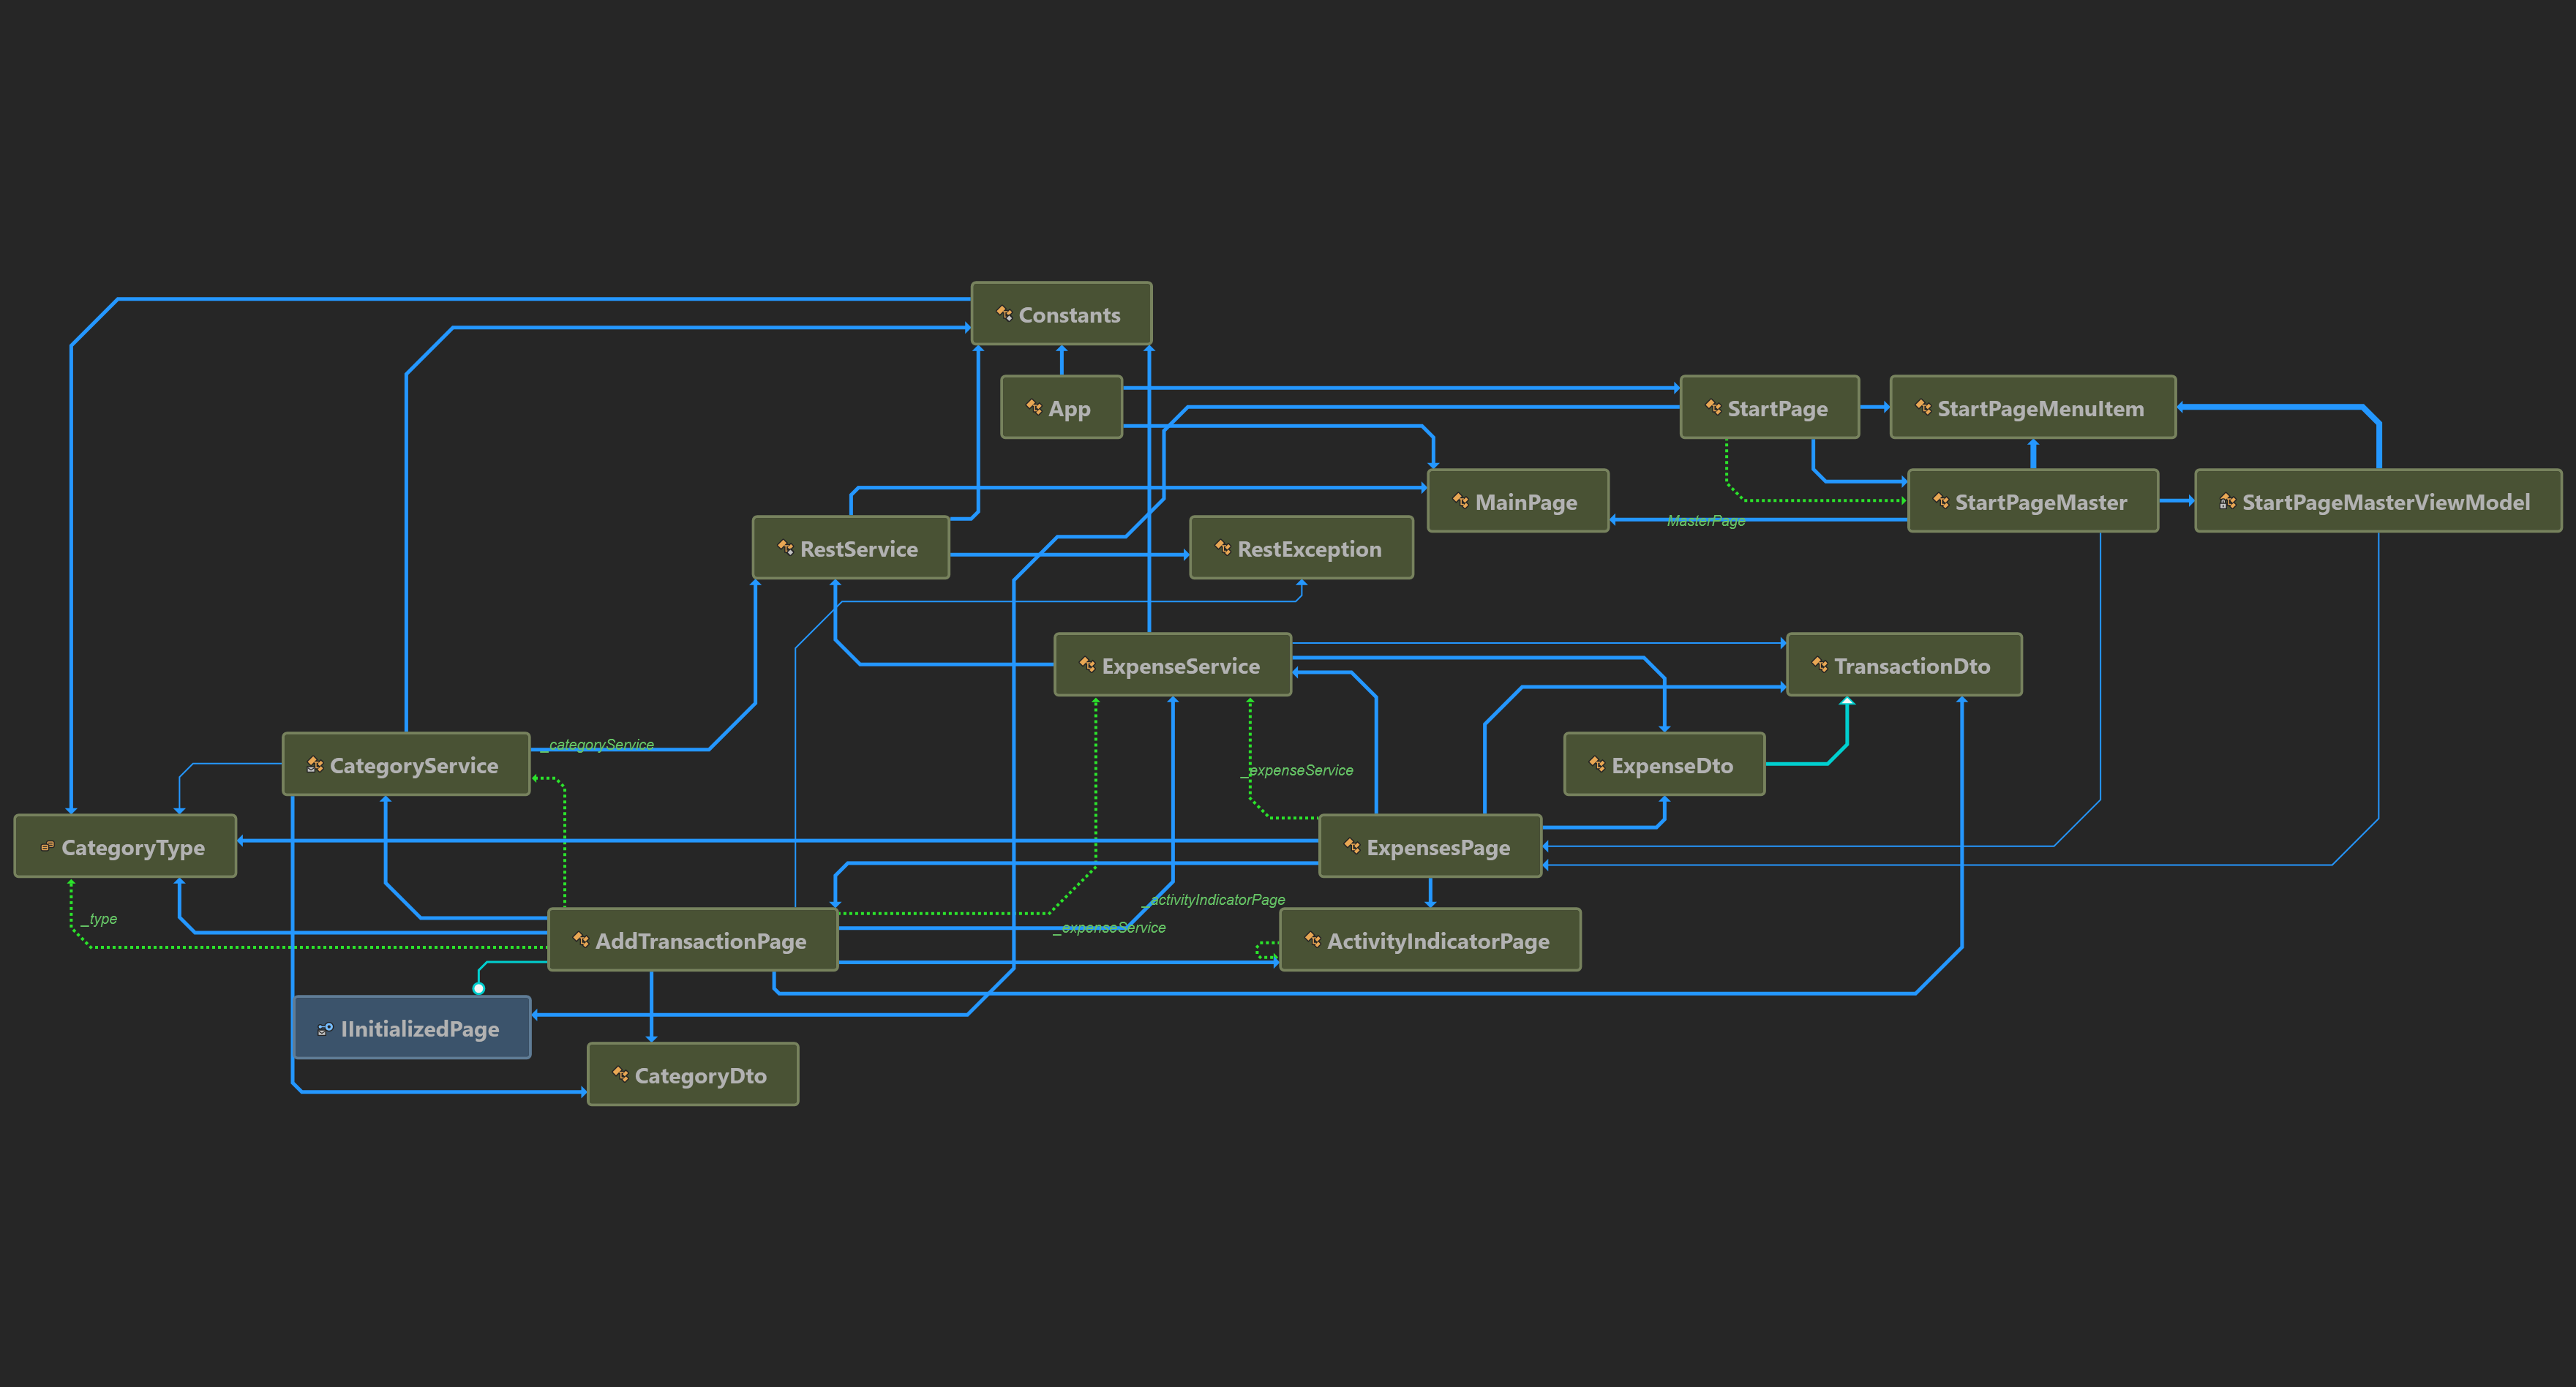
\includegraphics[width=6in]{img/diagram/interface_diagram.png}
		\caption{Diagram zależności typów warstwy logiki biznesowej dla modułu wydatków.}
		\label{xamarinexpenses}
	\end{center}
\end{figure}

Aplikacja obsługuje wszystkie akcje użytkownika wykonywane na stronach aplikacji przy użyciu serwisów, których zadaniem jest odczytanie danych wprowadzonych przez użytkownika i skonstruowanie zapytania do części serwerowej. Każde wysyłane zapytanie oprócz zapytań dotyczących rejestracji i logowania posiada dołączony nagłówek \lstinline|Authorization|, który zawiera token uwierzytelniający wygenerowany w części serwerowej aplikacji.

Dzięki zastosowaniu do komunikacji z częścią serwerową metod asynchronicznych interfejs użytkownika jest responsywny i podczas, gdy serwer przetwarza zapytanie wyświetlany jest stosowny wskaźnik oczekiwania.